\section{Torsors and principal bundles}

The classical theory of principal bundles tells us to look for an appropriate classifying space of torsors to map into. Homotopy type theory tells us that classifying spaces are univalent fibrations. The type of torsors is not a priori such a fibration, so we'll do some work to make that happen. This will constitute the codomain of the investigation.

\begin{mydef}
Let \( G \) be a group (a set with the usual classical structure and properties). A \defemph{\( G \)-set} is a set \( X \) equipped with a homomorphism \( \phi:G\to\Aut(X) \). If in addition we have a term
\[ 
\mathsf{is\_torsor}:||X||_{-1}\times \pit{g:G}\mathsf{is\_equiv}(\phi(-,x):G\to X)
\] then we call this data a \defemph{\( G \)-torsor}. Denote the type of \( G \)-torsors by \( TG \).
\end{mydef}

If \( (X,\phi),(Y,\psi):TG \) then a \( G \)-equivariant map is a function \( f:X\to Y \) such that \( f(\phi(g,x))=\psi(g,f(x)) \). Denote the type of \( G \)-equivariant maps by \( X\to_G Y \).

\begin{mylemma}
There is a natural equivalence \( (X=_{TG}Y) \simeq (X\to_G Y) \).\qed
\end{mylemma}

Denote by \( * \) the torsor given by \( G \) actions on its underlying set by left-translation. This serves as a basepoint for \( TG \) and we have a group isomorphism \( \Omega TG\simeq G \).

\begin{mylemma}
A \( G \)-set \( (X,\phi) \) is a \( G \)-torsor if and only if there merely exists a \( G \)-equivariant equivalence \( *\to_G X \).\qed
\end{mylemma}

\begin{mycor}
The pointed type \( (TG,*) \) is a \( \K(G,1) \).\qed
\end{mycor}

\subsection{Univalent replacement for torsors}

The homotopy type theory of cohomology and bundles tells us that the type of principal \( G \)-bundles on a type \( M \) is the type \( M\to\K(G,1) \). But this is a type of structured types, a connected component of \( G \)-sets rather than a connected component of the universe. The paths \emph{in the universe} between two \( G \)-sets is equivalent to the type of equivalences between the \emph{underlying types}, not just the equivariant equivalences. We wish to work with a connected component of the universe \( \uni \).

We'll resolve this problem with the following discussion, following Scoccola\cite{sco}. We will state the definitions and theorems for a general \( \K(G,n) \) but we will be focusing on \( n=1 \) in this note.

\begin{mydef}
Let \( \EM(G,n)\defeq \BAut(\K(G,n))\defeq \sit{Y:\uni}||Y\simeq \K(G,n)||_{-1}\). A \defemph{\( \K(G,n) \)-bundle} on a type \( M \) is the fiber of a map \( M\to\EM(G,n) \).
\end{mydef}

Scoccola uses two self-maps on the universe: suspension followed by \( (n+1) \)-truncation \( ||\Sigma||_{n+1} \) and forgetting a point \( F_\bullet \) to form the composition 
\[ 
\EM(G,n)\xrightarrow[]{||\Sigma||_{n+1}} \EM_{\bullet\bullet}(G,n+1)\xrightarrow[]{F_\bullet}\EMp(G,n+1)
\]
from types to types with two points (north and south), to pointed types (by forgetting the south point).

\begin{mydef}
Given \( f:M\to\EM(G,n) \), the \defemph{associated action of \( M \) on \( G \)}, denoted by \( f_\bullet \) is defined to be \( f_\bullet=F_\bullet\circ||\Sigma||_{n+1}\circ f \).
\end{mydef}

\begin{mythm}
(Scoccola\cite{sco} Proposition 2.39). A \( \K(G,n) \) bundle \( f:M\to\EM(G,n) \) is equivalent to a map in \( M\to\K(G,n+1) \), and so is a principal fibration, if and only if the associated action \( f_\bullet \) is contractible.
\end{mythm}

Let's relate this to \emph{orientation}. Note that the obstruction in the theorem is about a map into \( \EMp(G,n+1) \) and further note that \( \EMp(G,n)\simeq \K(\Aut G,1) \) (independent of \( n \)). The theorem says that the data of a map into \( \EM(G,n) \) factors into data about a map into \( \K(G,n+1) \) and one into \( \K(\Aut G,1) \). Informally, \( \EM(G,n) \) is a little too large to be a \( K(G,n+1) \), as it includes data about automorphisms of \( G \).

In the special case of \( \EMzo \) the conditions of the theorem are met when \( f_\bullet:M\to\K(\Aut \zz, 1) \) is contractible. \( \Aut\zz \) consists of the \( \zz/2\zz \) worth of outer automorphisms given by multiplication by \( \pm 1 \). Symmetries of the circle are our discrete stand-in for the matrix group \( O(2) \), which contains both rotations and (orientation-reversing) reflections of the plane. Requiring a contractible induced map to \( \pm 1 \) amounts to a choice of direction for all the circles, and so deserves the name ``\( f \) is \emph{orientable}.'' In addition \( f_\bullet \) deserves to be called the first Stiefel-Whitney class of \( f \), and the requirement here is that it vanishes. 

\begin{mynote}
Reinterpreting more of the theory of characteristic classes would be an enlightening future project. Defining a Chern class and Euler class in 2 dimensions is a goal of this note, but we will not prove all the various laws these classes satisfy (the Whitney sum formula and so on). Nonabelian matrix Lie groups such as \( SO(n) \) and \( SU(n) \) are not fully imported into homotopy type theory, but recall that some classical results from the theory of characteristic classes are obtained by replacing the group with a maximal torus, which should be a smaller leap from what is presented here\cite{splitting_principle}.
\end{mynote}

In summary, we can continue to work with the univalent fibration \( \EM(G,1) \) and still know that we are also studying principal \( \K(G,1) \)-fibrations, if the bundle is orientable.

\subsection{Pathovers in principal bundles}
Suppose we have \( T:M\to\EMzo \) and \( P\defeq\sit{x:M}T(x) \). We adopt a convention of naming objects in \( M \) with Latin letters, and the corresponding structures in \( P \) with Greek letters. Recall that if \( p:a=_M b \) then \( T \) acts on \( p \) with what's called the \emph{action on paths}, denoted \( \ap(T)(p):T(a)=T(b) \). This is a path in the codomain, which in this case is a type of types. Type theory also provides a function called \emph{transport}, denoted \( \tr_p:T(a)\to T(b) \) which acts on the fibers of \( P \). \( \tr_p \) acts on the terms of the types \( T(a) \) and \( T(b) \), and univalence tells us this is the isomorphism corresponding to \( \ap(T)(p) \).

Type theory also tells us that paths in \( P \) are given by pairs of paths: a path \( p:a=_M b \) in the base, and a pathover \( \pi:\tr_p(\alpha)=_{T(b)}\beta \) between \( \alpha:T(a) \) and \( \beta:T(b) \) in the fibers. We can't directly compare \( \alpha \) and \( \beta \) since they are of different types, so we apply transport to one of them. We say \( \pi \) lies over \( p \). See Figure~\ref{fig:pathovers}.

\begin{figure}[htbp]
\centering
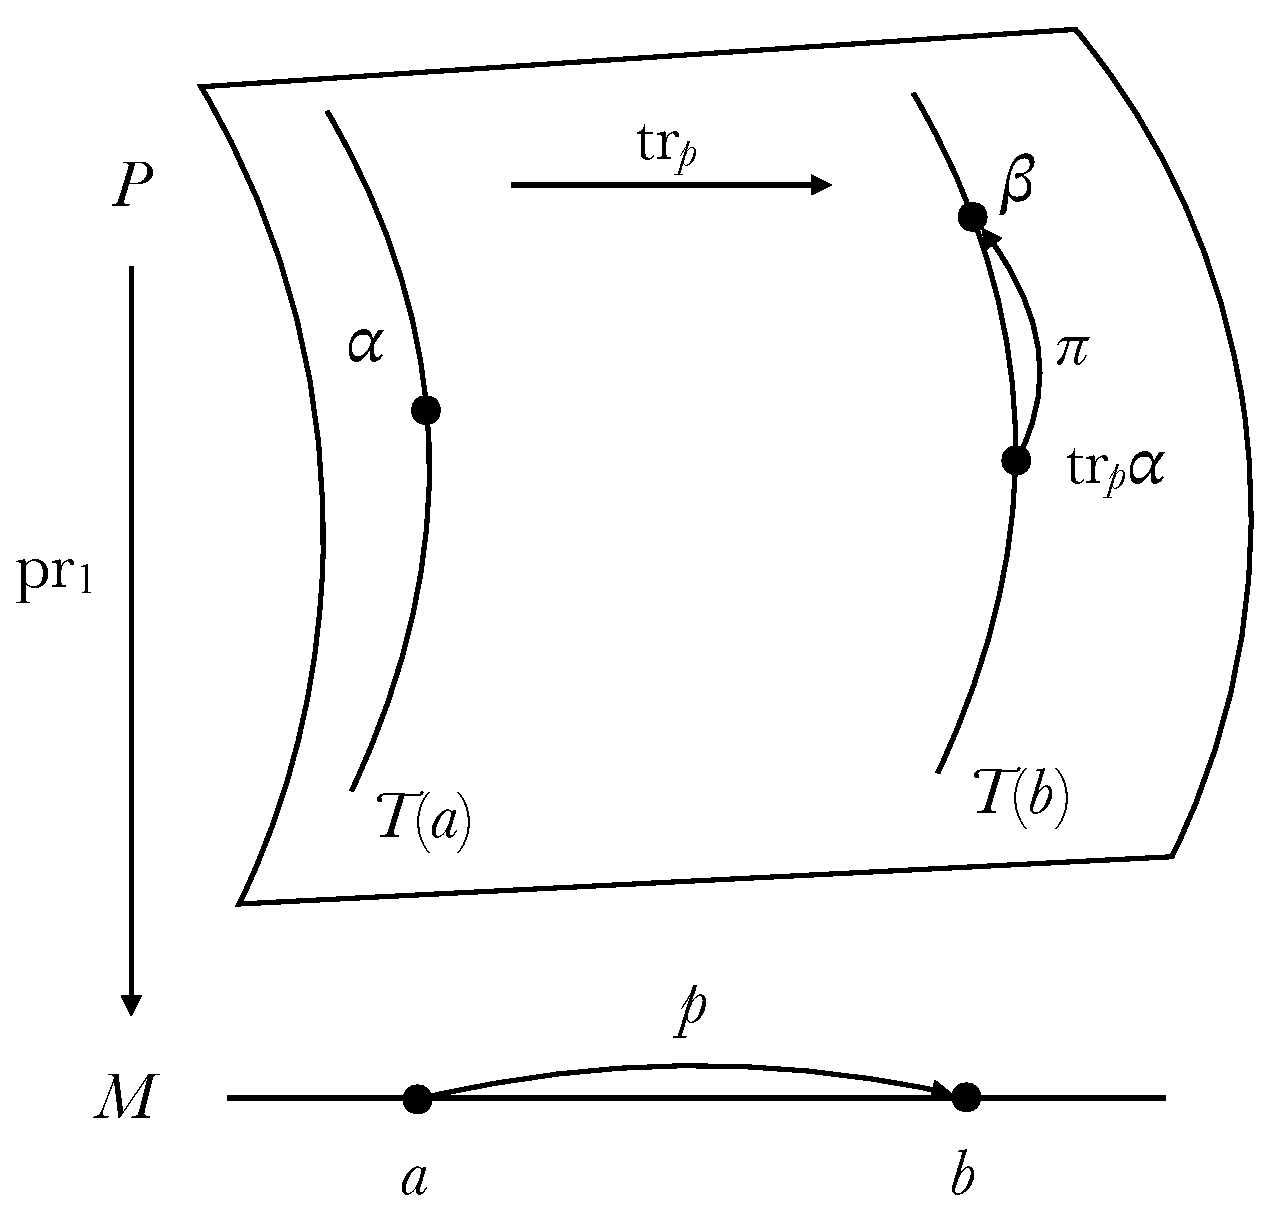
\includegraphics[width=200pt]{pathovers.pdf}
\caption{A path \( \pi \) over the path \( p \) in the base involves the transport function.}
\label{fig:pathovers}
\end{figure}

Lastly we want to recall that in the presence of a section \( s:M\to P \) there is a dependent generalization of \( \ap \) called \( \apd \): \( \apd_p(s):\tr_p(s(a))=s(b) \) which is a pathover between the two values of the section over the basepoints of the path \( p \).
